%% This is file `elsarticle-template-1-num.tex',
%%
%% Copyright 2009 Elsevier Ltd
%%
%% This file is part of the 'Elsarticle Bundle'.
%% ---------------------------------------------
%%
%% It may be distributed under the conditions of the LaTeX Project Public
%% License, either version 1.2 of this license or (at your option) any
%% later version.  The latest version of this license is in
%%    http://www.latex-project.org/lppl.txt
%% and version 1.2 or later is part of all distributions of LaTeX
%% version 1999/12/01 or later.
%%
%% Template article for Elsevier's document class `elsarticle'
%% with numbered style bibliographic references
%%
%% $Id: elsarticle-template-1-num.tex 149 2009-10-08 05:01:15Z rishi $
%% $URL: http://lenova.river-valley.com/svn/elsbst/trunk/elsarticle-template-1-num.tex $
%%
\documentclass[preprint,12pt]{elsarticle}

%% Use the option review to obtain double line spacing
%% \documentclass[preprint,review,12pt]{elsarticle}
\RequirePackage[usenames, dvipsnames]{xcolor}

%% Use the options 1p,twocolumn; 3p; 3p,twocolumn; 5p; or 5p,twocolumn
%% for a journal layout:
%% \documentclass[final,1p,times]{elsarticle}
%% \documentclass[final,1p,times,twocolumn]{elsarticle}
%% \documentclass[final,3p,times]{elsarticle}
%% \documentclass[final,3p,times,twocolumn]{elsarticle}
%% \documentclass[final,5p,times]{elsarticle}
%% \documentclass[final,5p,times,twocolumn]{elsarticle}

%% The graphicx package provides the includegraphics command.
\usepackage{graphicx}
%% The amssymb package provides various useful mathematical symbols
\usepackage{amssymb}
%% The amsthm package provides extended theorem environments
%% \usepackage{amsthm}

%% The lineno packages adds line numbers. Start line numbering with
%% \begin{linenumbers}, end it with \end{linenumbers}. Or switch it on
%% for the whole article with \linenumbers after \end{frontmatter}.
\usepackage{lineno}
\usepackage{xcolor}
\usepackage{multirow}
\usepackage{algorithm}%, algorithm2e}
\usepackage[noend]{algorithmic}

\usepackage{tikz, xcolor}
\usetikzlibrary{arrows,shapes, positioning, matrix, patterns}

%% natbib.sty is loaded by default. However, natbib options can be
%% provided with \biboptions{...} command. Following options are
%% valid:

%%   round  -  round parentheses are used (default)
%%   square -  square brackets are used   [option]
%%   curly  -  curly braces are used      {option}
%%   angle  -  angle brackets are used    <option>
%%   semicolon  -  multiple citations separated by semi-colon
%%   colon  - same as semicolon, an earlier confusion
%%   comma  -  separated by comma
%%   numbers-  selects numerical citations
%%   super  -  numerical citations as superscripts
%%   sort   -  sorts multiple citations according to order in ref. list
%%   sort&compress   -  like sort, but also compresses numerical citations
%%   compress - compresses without sorting
%%
%% \biboptions{comma,round}

% \biboptions{}

\journal{Journal XXX}

\begin{document}

\begin{frontmatter}

%% Title, authors and addresses

\title{When to use Hamming distance and k-mismatches algorithms using fast Fourier transform?}

%% use the tnoteref command within \title for footnotes;
%% use the tnotetext command for the associated footnote;
%% use the fnref command within \author or \address for footnotes;
%% use the fntext command for the associated footnote;
%% use the corref command within \author for corresponding author footnotes;
%% use the cortext command for the associated footnote;
%% use the ead command for the email address,
%% and the form \ead[url] for the home page:
%%
%% \title{Title\tnoteref{label1}}
%% \tnotetext[label1]{}
%% \author{Name\corref{cor1}\fnref{label2}}
%% \ead{email address}
%% \ead[url]{home page}
%% \fntext[label2]{}
%% \cortext[cor1]{}
%% \address{Address\fnref{label3}}
%% \fntext[label3]{}


%% use optional labels to link authors explicitly to addresses:
%% \author[label1,label2]{<author name>}
%% \address[label1]{<address>}
%% \address[label2]{<address>}

\author{Tatiana Rocher}

\address{University of Bristol, UK}

\begin{abstract}
%% Text of abstract
?????
\end{abstract}

\begin{keyword}
Hamming distance \sep fast Fourier transform
%% keywords here, in the form: keyword \sep keyword

%% MSC codes here, in the form: \MSC code \sep code
%% or \MSC[2008] code \sep code (2000 is the default)

\end{keyword}

\end{frontmatter}

%%
%% Start line numbering here if you want
%%
\linenumbers

%% main text
\section*{Introduction}
\label{S:1}

\textcolor{red}{not good}

The last decades saw a lot of algorithm improvement coming.
The expected time consumption is most of the time based on the algorithm's worst complexity.

We wanted to know if the k-mismatching algorithm of Gawrychowski and Uznanski \cite{Kmism3} could be used.
We decided to compare it to some of it predessessors.

We gathered 6 algorithms, responding to 4 problems.
Every algorithm responding to a problem were compared to the others and to the naive algorithm.

The section \ref{Algo} presents the selection of algorithms.
Then we explain in the section \ref{Method} our implementation procedure and the datasets we used.
Finally, the section \ref{Res} present our tests and results.



\section{Algorithms}
\label{Algo}

The algorithms use between $1$ and $3$ of the following methods: the FFT, Kangaroo or RLE methods.
All algorithms except the k-mismatching $1$ use the FFT method,
all k-mismatching use the Kangaroo method
and the k-mismatching $3$ uses the RLE method.
Those relations are summarized in the figure \ref{AllAlgorithms}.


\begin{figure}[h]\centering
\begin{tikzpicture}[scale=1.5, every node/.style={scale=1.5}]
% \documentclass{standalone}
% \RequirePackage[usenames, dvipsnames]{xcolor}
% \usepackage{tikz, xcolor}
% \usetikzlibrary{arrows,shapes, positioning, calc, matrix, decorations.pathreplacing}


\newcommand{\test}{
\tikzset{
indice/.style={scale=0.7, align=center},
fleche/.style={->, >=stealth'},
case1/.style={rounded corners=6pt, line width=0.7pt, draw=NavyBlue}, 
case2/.style={rounded corners=6pt, line width=0.7pt, draw=YellowOrange}
}

\node[indice] at (0, 0) (fft) {FFT\\method};
\draw[case1] (fft.north west) rectangle (fft.south east);
% \draw[draw=blue] (fft) ellipse (20pt and 10pt);
\node[below=1.5cm of fft] (b) {};
\node[left=1cm of b, indice] (wc) {Wildcard\\matching};
\draw[case2] (wc.north west) rectangle (wc.south east);
% \draw (wc) ellipse (20pt and 10pt);
\node[right=-0.3cm of b, indice] (ehd) {Exact\\Hamming\\distance};
\draw[case2] (ehd.north west) rectangle (ehd.south east);
% \draw (ehd) ellipse (20pt and 13pt);
\node[below=0.9cm of ehd, indice] (ahd) {Approx.\\Hamming\\distance};
\draw[case2] (ahd.north west) rectangle (ahd.south east);
% \draw (ahd) ellipse (20pt and 13pt);

\node[right=5.5cm of fft, indice] (lcp) {Kangaroo\\method};
\draw[case1] (lcp.north west) rectangle (lcp.south east);
\node[right=1.2cm of lcp, indice] (rle) {RLE\\method};
\draw[case1] (rle.north west) rectangle (rle.south east);
% \draw[draw=blue] (lcp) ellipse (20pt and 9pt);
\node[below=1.2cm of lcp, indice] (kmism3) {K-mism.\\3};
\draw[case2] (kmism3.north west) rectangle (kmism3.south east);
% \draw (kmism1) ellipse (18pt and 9pt);
\node[left=1.2cm of kmism3, indice] (kmism2) {K-mism.\\2};
\draw[case2] (kmism2.north west) rectangle (kmism2.south east);
% \draw (kmism2) ellipse (18pt and 9pt);
\node[right=1.2cm of kmism3, indice] (kmism1) {K-mism.\\1};
\draw[case2] (kmism1.north west) rectangle (kmism1.south east);
% \draw (kmism3) ellipse (18pt and 9pt);

\draw[fleche] (wc) -- (fft);
\draw[fleche] (ehd) -- (fft);
\draw[fleche] (ahd) -- (ehd);
\draw[fleche] (kmism1) -- (lcp);
\draw[fleche] (kmism2) -- (lcp);
\draw[fleche] (kmism2) -- (fft);
\draw[fleche] (kmism3) -- (lcp);
\draw[fleche] (kmism3) -- (rle);
\draw[fleche] (kmism3) -- (fft);
}


% \begin{document}
% \begin{tikzpicture}
%   \test
% \end{tikzpicture}
% \end{document}
\test
\end{tikzpicture}
\caption{
The methods are in blue, the algorithms in orange.
A link indicates that the algorithm uses the linked method (or algorithm).
}\label{AllAlgorithms}
\end{figure}

We will present the three methods, and the algorithms.


\subsection{FFT method}

The fast Fourier transform (FFT) can be used to have the result of the multiplication of two vectors.
To do so, we compute the FFT of both vectors,
add the FFT,
then compute the inverse FFT of the result.

This multplication is helpfull in pattern matching algorithm,
see Algorithm \ref{MethodFFT}.
We compute two bit vectors matching the text and pattern
such that a $1$-bit appears when the letter $\alpha$ does,
do the FFT multiplication for the text and the inverse pattern,
the result shows the number of matching $\alpha$ at every alignment.

This method runs in $O(n \log n)$ times (for one letter).

\textcolor{red}{division en blocs de taille $2m$ partout}

\begin{algorithm}
\caption{$HD\_FFT(T, P, \alpha)$: }
\label{MethodFFT}
\begin{algorithmic}[1]
\REQUIRE T of size $n$, P of size $m$
\STATE init $B_t[n]$, $B_p[m]$ \COMMENT {\texttt{bit vectors}}
\STATE init $Res[n]$
\FOR {$i$ from $0$ to $n$} 
	\STATE {$B_t[i] == \alpha? B_t[i] = 1 : B_t[i] = 0$} 
\COMMENT {\texttt{Match every }$\alpha$ \texttt{letter of }$T$}
	% \STATE $B_t[i] = 1$ 
	% \ELSE
	% \STATE $B_t[i] = 0$
	% \ENDIF
\ENDFOR
\FOR {$i$ from $0$ to $m$} 
	\STATE {$B_p[i] == \alpha? B_p[i] = 1 : B_p[i] = 0$}  \COMMENT {\texttt{Match every $\alpha$ letter of $P$}}
	% \IF {$B_p[i] == \alpha$}
	% \STATE $B_p[i] = 1$
	% \ELSE
	% \STATE $B_p[i] = 0$
% \ENDIF
\ENDFOR
\STATE $FFT_t = FFT(B_t)$ \COMMENT {\texttt{Compute the FFT of $B_t$}}
\STATE $FFT_p = FFT(B_p)$
\STATE $FFT_r = FFT_t + Reverse(FFT_p)$
\STATE $Res = InvFFT(FFT_r)$ \COMMENT {\texttt{Compute the inverse FFT}}
% % \ENDFOR
\RETURN $Res$

\end{algorithmic}
\end{algorithm}



\subsection{Exact Hamming distance}
\label{eHD}

cite \cite{ExactHD}

The FFT method can be used for every unique letter of the pattern, and adding the temporary results.
Then for each position, we deduct this result from the pattern size to have the Hamming distance.
This algorithm runs in $O(n|\Sigma| m \log n)$ times
(in $O(n|\Sigma| m \log m)$ if we divide the text in blocs of size $2m$).

A way to optimize this algorithm is to put a threshold $\ell = \sqrt{m \log n}$
to sort the pattern letters as frequent or infrequent,
where a frequent letter appears more than $\ell$ times in the pattern.
The FFT method is used on the frequent letters.
We initialize a vector $A$, and do a single read of the text:
if we read an infrequent letter $\alpha$ at position $i$, we increment $A[i-k]$,
where $k$ is every occurrence of $\alpha$ in the pattern.
See algorithm \ref{ExHD}.
This algorithm runs in $O(n \sqrt{m} \log m)$ times.


\textcolor{red}{Q: Do we write every algorithm this way: pseudo-code and explanation?}


\begin{algorithm}
\label{ExHD}
\caption{$ExHD(T, P)$: Compute the exact Hamming distance between $T$ and $P$}
\begin{algorithmic}
\REQUIRE {$T$ of size $n$, $P$ of size $m$, $\Sigma$}
\STATE init $Res[n-m+1]$, $cpt[\Sigma]$
\STATE $\ell = sqrt(m \log n)$
\STATE $CountLetters(P, \ell)$ \COMMENT {$O(m)$}
\FOR {every $\alpha$ in $\Sigma$}
	\IF {$isFrequent(\alpha)$}
		\STATE $Tmp = HD\_FFT(T, P, \alpha)$
		\FOR {$i$ in $[0, n-m+1]$}
			\STATE $Res[i] += Tmp[i]$
		\ENDFOR
		\ENDIF
\ENDFOR
\FOR {$i$ in $[0, n]$}
	\IF {$isInfrequent(T[i])$}
		\FOR {all $P[k] == T[i]$}
			\STATE $Res[i - k]++$ \COMMENT {positions $k$ are precomputed during $CountLetters$}
		\ENDFOR
	\ENDIF
\ENDFOR
\FOR {$i$ in $[0 ,n]$}
	\STATE $Res[i] = m - Res[i]$
\ENDFOR
\RETURN $Res$

\end{algorithmic}
\end{algorithm}




\subsection{Approximate Hamming distance}

Kopelowitz and Porat \cite{ApproxHD} proposed an algorithm to approximate the Hamming distance
using the exact Hamming distance algorithm, see section \ref{eHD}.
For a $1 \pm \epsilon$ approximation,
the algorithm runs $c+\log m$ iterations of the following loop:
\begin{itemize}
\setlength\itemsep{0.1em}
\item find a random mapping on $2 / \epsilon$ letters
\item compute the Hamming distance of $T$ and $P$, both mapped on this alphabet
\item keep  the bigger value for every position
\end{itemize}

This algorithms runs in $O(n / \epsilon \log n \log m)$ times.
See algorithm \ref{AppHD}.


\begin{algorithm}
\label{AppHD}
\caption{$AppHD(T, P, \epsilon)$: Compute an $(1 \pm \epsilon)$ approximate Hamming distance between $T$ and $P$}
\begin{algorithmic}

\REQUIRE {$T$ of size $n$, $P$ of size $m$, $\Sigma$, $\epsilon$}
\STATE init Res
\FOR {$i$ in $0, c * \log m]$}
	\STATE $Map = RandomMapping(\Sigma, 2 / \epsilon)$
	\STATE $Tmp = ExHD(Map(T), Map(P))$
	\FOR {$j$ in $[0, n-m+1]$}
		\IF {$Tmp[j]>Res[j]$}
			\STATE $Res[j]=Tmp[j]$
		\ENDIF
	\ENDFOR
\ENDFOR
\RETURN Res

\end{algorithmic}
\end{algorithm}




\subsection{Exact wildcard matching}

In $2006$, Clifford and Clifford \cite{WC}, proposed an algorithm to solve
exact matching with wildcards.
Here, every letter is replaced by a number, with $0$ beeing a wildcard.

The idea is to compute the sum of squared differences between the text and pattern
(\textcolor{red}{and multiply by the XXX} ) at every alignment.
We use the pattern and text's FFTs, and theirs squared and cubed FFTs:
$FFT^2_P$ is the pattern's FFT where all its coefficient are the cubed coefficient of $FFT_P$.
The algorithm computes: 
\begin{itemize}
\setlength\itemsep{0.1em}
\item $a = FFT_T+ FFT^3_P$
\item $b = FFT^2_T+ FFT^2_P$
\item $c = FFT^3_T+ FFT_P$.
\item $Res = InvFFT(a) - 2*InvFFT(b) + InvFFT(c)$
\end{itemize}

Every position $i$ where $Res[i] = 0$ is an exact matching.
This algorithms runs in $O(n \log m)$ times. See algorithm \ref{WC}.



\begin{algorithm}
\label{WC}
\caption{$WC(T, P)$: Find where $P$ matches in $P$}
\begin{algorithmic}

\REQUIRE {$T$ of size $n$, $P$ of size $m$}
\STATE Compute $FFT_T$ and $FFT_P$
\STATE Compute $FFT^2_T$, $FFT^3_T$, $FFT^2_P$ and $FFT^3_P$ \COMMENT {in $O(n)$ and $O(m)$}
\STATE $a = FFT_T+ FFT^3_P$
\STATE $b = FFT^2_T+ FFT^2_P$
\STATE $c = FFT^3_T+ FFT_P$
\STATE $Res = InvFFT(a) - 2*InvFFT(b) + InvFFT(c)$
\RETURN $Res$

\end{algorithmic}
\end{algorithm}


\subsection{Kangaroo method}

The Kangaroo method uses the longest common prefix (LCP) between two words.
It needs a structure which returns the LCP between any suffix of the text and any suffix of the pattern
in $O(1)$ times.

cite qui ????

For every position $i$ in $T$, the Kangaroo method finds the LCP between $T$ and $P$
starting at $T[i]$ and $P[0]$.
Let says this LCP is of length $p$, we have $T[i+p] \neq P[p]$.
Then the method looks for the following LCP starting at position $T[i+p+1]$ and $P[p+1]$.
We have the Hamming distance if we look for the LCP until we reach the end of the pattern.
% This method runs in $O(nm)$ times.

\textcolor{red}{vérifier que se soit bien ça !!}

\textcolor{red}{I put the kangaroo and RLE methods here so they are close to the algorithms using them.}


\subsection{K-mismatching 1}

This algorithm\cite{Kangaroo} uses the Kangaroo method:
for every position in $T$, it looks for the LCP up to $k$ times or until we reach the end of the pattern.

This algorithm runs in $O(kn)$ times, see algorithm \ref{K1}.



\begin{algorithm}
\label{K1}
\caption{$K\_mism\_1(T, P, k)$}
\begin{algorithmic}

\REQUIRE {$T$ of size $n$, $P$ of size $m$, $k$}
\STATE init $Res[n-m+1]$
\STATE init $Struct\_LCP$
\FOR {$i$ in $[0, n-m+1]$}
	\STATE $pos_T = i$
	\STATE $pos_P = 0$
	\STATE $e=0$
	\WHILE {$e <=k$ OR $pos_P < m$}
		\STATE $p = FindLCP(pos_T, pos_P)$
		\STATE $pos_T += p + 1$
		\STATE $pos_P += p +1$
		\STATE $e++$
		\ENDWHILE
	\STATE $Res[i] = e$
\ENDFOR
\RETURN $Res$

\end{algorithmic}
\end{algorithm}


\subsection{K-mismatching 2}
Amir, Lewenstein and Porat\cite{Kmism2} proposed a k-mismatching algorithm
using both the FFT and Kangaroo methods.
This algorithm starts by sorting the pattern's letters as frequent or infrequent,
where a frequent letter appears more than $\sqrt{k}$ times.

If there is less than $2\sqrt{k}$ frequent letters: 
we use the FFT method with all the frequent letters and count the matching on infrequent letters directly.

If there is more than $2\sqrt{k}$ frequent letters:
We select $\sqrt{k}$ occurrences of $2\sqrt{k}$ frequent letters,
theirs positions gathered in a list $J$.
We initialise a vector $d$.
Then, for each position $i$ in $t$ and $j$ in $J$, such than $T[i] = P[j]$,
we increase $d[i-j]$.
For each position $i$ such that $d[i]>k$, we use the Kangaroo method.

This algorithm runs in $O(n\sqrt{k} \log k)$ times.


% \begin{algorithm}
% \label{K2}
% \caption{$K\_mism\_2(T, P, k)$}
% \begin{algorithmic}

% \REQUIRE {$T$ of size $n$, $P$ of size $m$, $k$}
% \STATE init $Res[n-m+1]$
% \STATE $SortLetters(P, 2\sqrt{k})$ \COMMENT {$O(m)$}
% \IF {$nbFreqLetters < 2*\sqrt{k}$}
% 	\FOR {every $\alpha$ in $frequentLetters$}
% 		\STATE $Tmp = HD\_FFT(T, P, \alpha)$
% 		\FOR {$i$ in $[0, n-m+1]$}
% 			\STATE $Res[i] += Tmp[i]$
% 		\ENDFOR
% 	\ENDFOR
% 	\FOR {$i$ in $[0, n]$}
% 		\IF {$isInfrequent(T[i])$}
% 			\FOR {all $P[k] == T[i]$}
% 				\STATE $Res[i - k]++$ \COMMENT {positions $k$ are precomputed during $CountLetters$}
% 			\ENDFOR
% 		\ENDIF
% 	\ENDFOR
% \ELSE
% 	\STATE init Struct\_LCP
% 	\STATE init $J$
% 	\FOR {$j$ in $[0, m]$}
% 		\IF {}
% 			\STATE $J.add[j]$
% 		\ENDIF
% 	\ENDFOR
% 	\FOR {$i$ in $[0, n]$}
% 		\FOR {}

% 		\ENDFOR
% 	\ENDFOR

% \ENDIF

% \RETURN $Res$

% \end{algorithmic}
% \end{algorithm}





\subsection{RLE method}

Let $T_{RLE}$ and $P_{RLE}$ be the run length encoding of $T$ and $P$.
This method uses every pair of text-pattern runs of the same letter
to update the second derivative of the Hamming distance,
see Algorithm \ref{RLEmet}.

The methods runs in \textcolor{red}{???XXX} times.


\begin{algorithm}
\label{RLEmet}
\caption{$K\_mism\_1(T, P, k)$}
\begin{algorithmic}

\REQUIRE {$T$ of size $n$, $P$ of size $m$, $k$}
\STATE init $A[n-m+1]$
\FOR {every run $r$ in $T_{RLE}$}
	\FOR {every run $s$ in $P_{RLE}$}
		\IF {$r.letter == s.letter$}
			\STATE $A[r.begin - s.end] ++$
			\STATE $A[r.end-s.end+1] --$
			\STATE $A[r.begin - s.begin+1]--$
			\STATE $A[r.end - s.begin +2] ++$
		\ENDIF
	\ENDFOR
\ENDFOR
\STATE $Res[0] = HD(T, P, 0)$
\STATE $Res[1] = HD(T, P, 1)$
\FOR {$i$ in $[2, n-m+1]$}
	\STATE $Res[i] = -A[i] + 2 * Res[i-1] - Res[i-2]$
\ENDFOR
\RETURN $Res$

\end{algorithmic}
\end{algorithm}






\subsection{K-mismatching 3}
Gawrychowski and Uznanski\cite{Kmism3} proposed the last k-mismatching algorithm of our selection.
It uses the FFT, Kangaroo and RLE methods. 

First, run a $(1 \pm \epsilon)$ approximate algorithm on the pattern against itself
to find a $O(k)$-period of the pattern.

If there is no $4k$-period smaller than $k$,
we run the $(1 \pm \epsilon)$ approximate algorithm on the pattern against the text
wz save the positions where the algorithm reports at most $k$ mismatches,
and we use the LCP method on this positions. 

If there is, we have $l$, the minimal $8k$-period of $P$.
we compute $P^*$ and $T^*$, the run length encoding of the reorganisation of $P$ and $T$ using $l$
(see \cite{Kmism3} for further explanations).
We sort the characters of $P^*$ as frequent or infrequent characters,
where $\alpha$ is a frequent character if it appears in more than $t$ runs
($t$ is undetermined in the paper).
We use a FFT for every frequent character,
and use the RLE method on infrequent characters.

This algorithm runs in $O(m \log^2 m \log |\Sigma| +k \sqrt{m \log m} * n/m)$ times.


\textcolor{red}{no algorithm here!}

\section{Method}
\label{Method}

All the algorithms were implemented in C++.

We compared $8$ methods from $3$ libraries to find how to do the fastest FFT multiplication:
AlgLib (free edition) \cite{alglib}, FFTW3 \cite{FFTW05} and Flint \cite{Hart2010}.
The AlgLib and FFTW3 libraries compute the FFT for two vectors,
adds the results and computes the inverse FFT of the result.
The Flint library computes a polynomial multiplication.
We tested the execution time of every method on vectors of $1$ million random integers.

The table \ref{tempsFFT} presents the average time of 10 executions.


\begin{table}[h]
\label{tempsFFT}
\begin{tabular}{|c|c|c|}
\hline
Library 				& Function used 							& Execution time (s) \\ \hline
AlgLib 					& fftr1d 									& $0.51$ \\ \hline
\multirow{2}{*}{FFTW3} 	& FFTW\_plan\_dft\_r2c\_1d (without saved plan) & $0.14$ \\
						& FFTW\_plan\_dft\_r2c\_1d (with saved plan) 	& $0.1$ \\ \hline
\multirow{5}{*}{Flint} 	& fmpz\_poly\_mul 							& $0.24$ \\
						& fmpq\_poly\_mul 							& $0.24$ \\
						& fq\_poly\_mul\_classical 					& $> 100$ \\
						& fq\_poly\_mul\_reorder 						& $1.17$ \\
						& fq\_poly\_mul\_KS 							& $1.50$ \\ \hline
\end{tabular}
\caption{Execution time of \textcolor{red}{XXXX}}
\end{table}

We choose to use the FFTW3 library.
FFTW3 uses a \textit{plan} which find the best method to compute the FFT of a given size.
A plan can be precomputed, saved and reused later.
Its documentation recommends to use FFT for vector which size is a power of $2$.
We computed and saved all FFT plans from $1$ number to $16$ millions numbers for our futur uses.
Except if specified, all runs used the patient flag.


\subsection{dataset}

The tests were made on real data:
\begin{itemize}
\setlength\itemsep{0.1em}
\item a DNA file composed of the full genome e.coli (4.6 Mb)
\item an English text composed of five books from the Sherlock Holmes serie from Sir Arthur Conan Doyles (8 Mb)
\end{itemize}
For the tests using this files, the text was a prefixe of the wanted size, 
the pattern was extracted from the file at a random position. \textcolor{red}{XXbaaad!!XX}

For some tests, we made artificial texts to force a characteristic.
Each one will be described in the result section.




\section{Results}
\label{Res}

Those tests were made in a computer Intel® Core™ i7-6700 CPU @ $3.40$GHz.

\textcolor{red}{what do we tell here ?}

Each algorithm was compared with at least a naive algorithm.





\subsection{exact matching using Wildcard}
\label{WCTests}

We want to know how to use the FFT method:
should we divide the text in substrings?
How much time do we save by using the saved plan?

This algorithm was tested on randomly generated files of numbers from $0$ to $10$.
The text was composed of $8$ millions numbers and the pattern of $100$ thousand numbers.
The naive algorithm runs in more than $10$ minutes.

The algorithm ran several times with several options:
when the text is computed fully or divided in blocs of size $2m$
and with or without charging the saved plan (with the patient flag).
Note that is we don't use a saved plan, the algorithm creates a plan with the estimate flag.
The table \ref{TableWC} shows the execution times with every option.

\begin{table}[h]
\begin{tabular}{|c|c|c|}
\hline
			& without saved plan & with saved plan \\ \hline
full text	& $7.84$ s & $5.95$ s \\ \hline
text divided in blocs of size $2m$ &  $5.83$ s & $5.59$ s \\ \hline
\end{tabular}
\caption{Excecution times of the exact matching using wildcards algorithm with several options.}
\label{TableWC}
\end{table}


Note that the plans with the patient flag were computed in
$90$ minutes for a FFT of $8$ millions letters
and in $33$ seconds for a FFT for $200$ thousands letters.

This algorithm runs faster if the text is divided in smaller blocs
and obviously if we use a plan already computed.

In the other hand, if the patient plan wasn't precomputed,
it is better to not force the algorithm to use a plan with a patient plan.
Moreover, it is often faster to compute a small plan with the exhaustive flag
than a bigger one with the patient flag, making the execution even faster.
In the example above, we could pre-compute the plan
with the exhaustive flag for $200$ thousand letters faster than
the plan with the patient flag for $8$ million letters ($3$ minutes to $90$ minutes).
The algorithm execution time using the exhaustive flag on $200$ thousand letters is $5.39$ seconds.

\subsubsection*{Algorithm utilisation}

Our naive algorithm computes the calculation $P[i] \times T[j] \times (T[j]-P[i])^2$,
for every position of every alignment between $T$ and $P$.
For a text of $8$ millions numbers and a pattern of $100$ thousand numbers,
the naive algorithm runs in more than $10$ minutes.

Our tests showed that the Wildcard algorithm is always faster than the naive algorithm, even in small texts.





\subsection{exact Hamming distance}


For a $8$ millions letters text and a $20$ thousands letters pattern, 
the algorithm runs in $4.1$ seconds on DNA sequences and in $5.7$ seconds on an English text.
% Can it be faster ?

We want to test:
\begin{itemize}
\setlength\itemsep{-0.4em}
\item how does the execution time vary with the pattern's form
\item how good is the threshold
\item what is the best threshold on real text
\end{itemize}

\textcolor{red}{Manque : quel temps d'execution après les modifications ??}



\subsubsection*{Pattern variation and execution time}

The algorithm is composed of two sections.
In the first section, the computation time depends
on the number of frequent letters in the pattern.
In the second section, the computation time depends on the number
of infrequent letters in the pattern and how often they appear in the text.

We want to know how the execution time can vary with the pattern,
so %for several sizes of pattern,
we made artificial patterns
with a minimum or maximum number of infrequent letter,
and inducing the computation of a defined number of FFT.
Let $L$ be the threshold with $L = sqrt(m \log n)$.
In a pattern with the minimum number of infrequent letters ($0$),
all letters will appear more than $L$ times
(we use $m/\sigma$ occurrences for each letters).
In a pattern with the maximum number of infrequent letters,
we want to maximize the occurrences $k'$ of each infrequent letter
while still having the number of frequent letter we want.
We want the greater $k'<L$ such that $k > L$,
where $k$ in the number of occurrence of each frequent letter.
% We have:
% every frequent letter appear $k= max(L, (m - (L-1)* \sigma-X)/X)$
% every infrequent letter appear $(m-k*X)/(\sigma -X)$,
% such that $X$ is the number of frequent letters and $\sigma$ is the number of letters in the alphabet.

We ran the algorithm in patterns of increasing size (up to $20 000$ letters) inducing $1$ to $4$ FFT,
with a minimum and maximum number of frequent letters, with $\sigma = 4$ (as a DNA pattern)
and $\sigma = 95$ (as an English pattern).
We also ran the algorithm when every letters of the pattern occur equally and $L=m$ such that no FFT is used.

The figure \ref{ExHDADN} presents the computation times on a $8$ millions letters DNA text.
The figure \ref{ExHDEnglish} presents the computation times on a $8$ millions English text.
The following times include the computation time without the initialisation and the writing in the output.
In this figures, a colored area indicates the expected execution time for a defined number of frequent letter.

\begin{figure}[h]
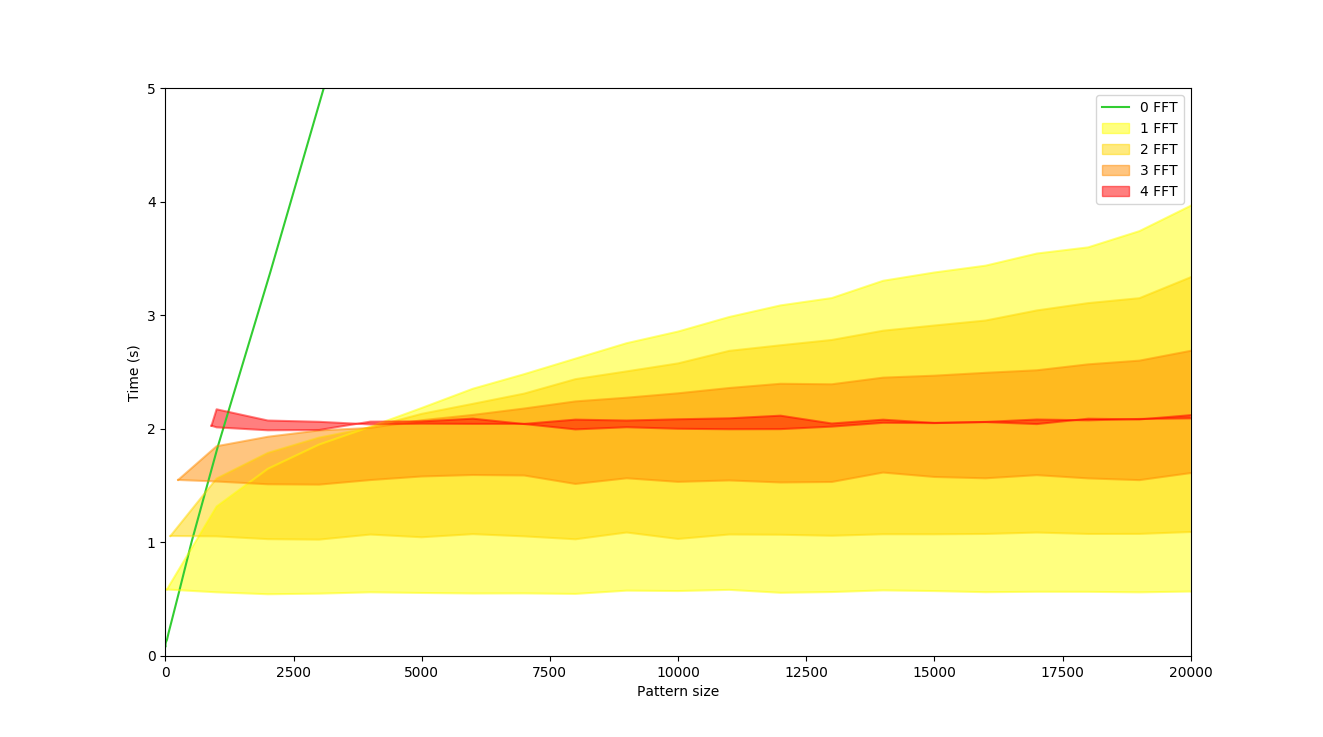
\includegraphics[scale=0.45]{./figures/ExHDADN.png}
\caption{DNA text of $8$ millions letters and DNA pattern of $0$ to $20 000$ letters, .
Execution time for $0$ to $4$ frequent letters.}
\label{ExHDADN}
\end{figure}

\begin{figure}[h]
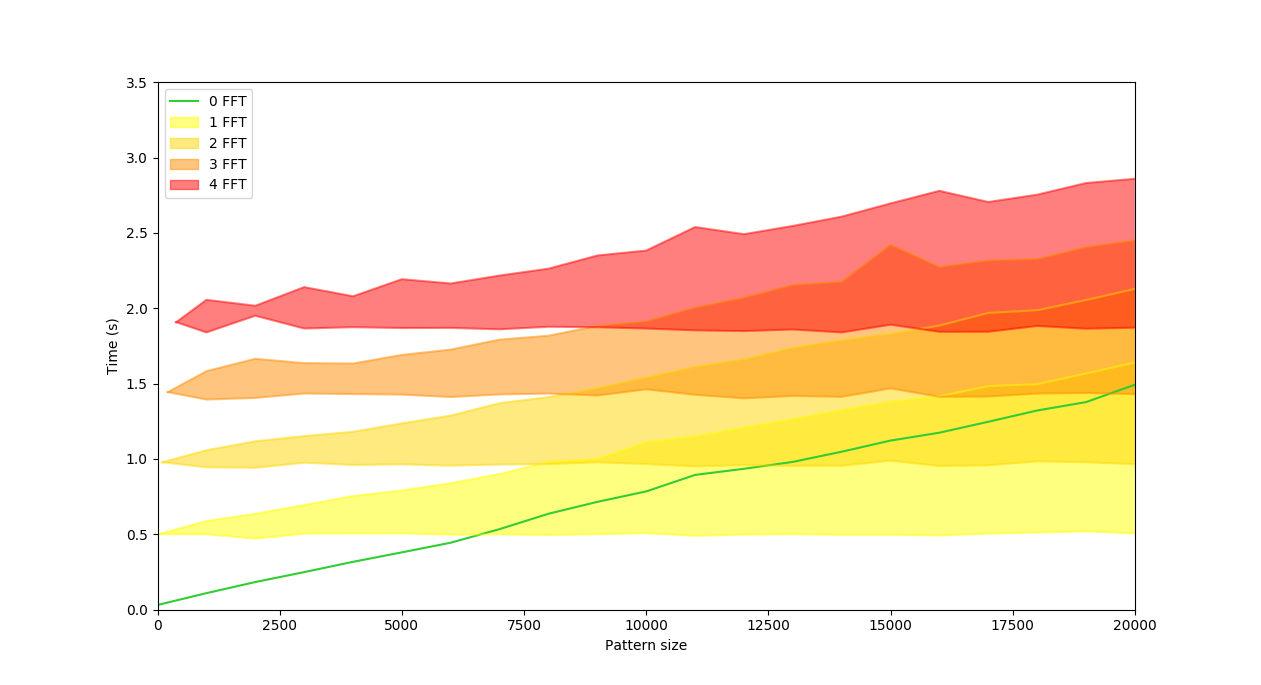
\includegraphics[scale=0.45]{./figures/ExHDEnglish.png}
\caption{English text of $8$ millions letters and English pattern of $0$ to $20 000$ letters.
Execution time for $0$ to $4$ frequent letters.}
\label{ExHDEnglish}
\end{figure}


The algorithm always benefits of the use of at least one FFT when the pattern is longer than $1500$ letters.
As there are only $4$ letters in a DNA pattern,
the computation time doesn't change when the pattern length increase with $4$ frequent letters.

In a pattern matching on real DNA sequence, the $4$ letters appear with almost the same amount of occurrencies.
In those cases,
the algorithm will use $4$ FFT and will run in $2$ seconds
for a $8$ millions letters text and every size of pattern.

In a English text and pattern, it is more interesting to not use any FFT for a pattern smaller than $6000$ letters.

The curve for the utilisation of $0$ FFT (in green) increases more slowly than the one in the DNA sequences.
This is due to the number of occurrences of each infrequent letters.
Assume that every infrequent letter appear with the same amount of occurrences.
In a English pattern, each $95$ letters appear $k'=m/95$ times,
while the $4$ DNA letters appear $k'=m/4$ times.
In the infrequent section, the algorithm looks for every pattern occurrences of the letters of each position,
thus $k'*m$ calculations:
we have $m^2/95$ calculations in the English text,
and $m^2/4$ calculations in the DNA text. 

The same idea is used to explain the difference between the maximal curves in the English and DNA texts.

% In a pattern matching on real English text, a few FFT are usually made, for example the characters space, carriage return, 'e'\ldots
% \textcolor{red}{what do I want to say with that ?}

The tests indicate a large variability of computation times.
If we don't know the letters' repartition as frequent or infrequent,
the hamming distance between a English text of $8$ millions letters
and a pattern of $20 000$ letters can be computed between $0.5$ s and $2.8$ seconds
(for up to $4$ FFT).
The threshold may be badly chosen and could be updated by considering the real FFT computation time.




\subsubsection*{Which pattern should we use while using real DNA or English texts?}

To find the best threshold to use,
we selected an English text of $8$ million letters
and ran the algorithm several times
with a $20 000$ letters pattern
randomly extracted from the text at each run.
We increased the threshold from $400$ to $2500$ letters occurrences.% with a 100 letters steps.

The results are gathered in the figure \ref{ExHDThresh} where
every point represents a run and its colour indicates the number of FFT used.
The line is the average computation time of $10$ runs.
It is used to find the best threshold:
the one inducing the smaller computation time.


\begin{figure}[h]
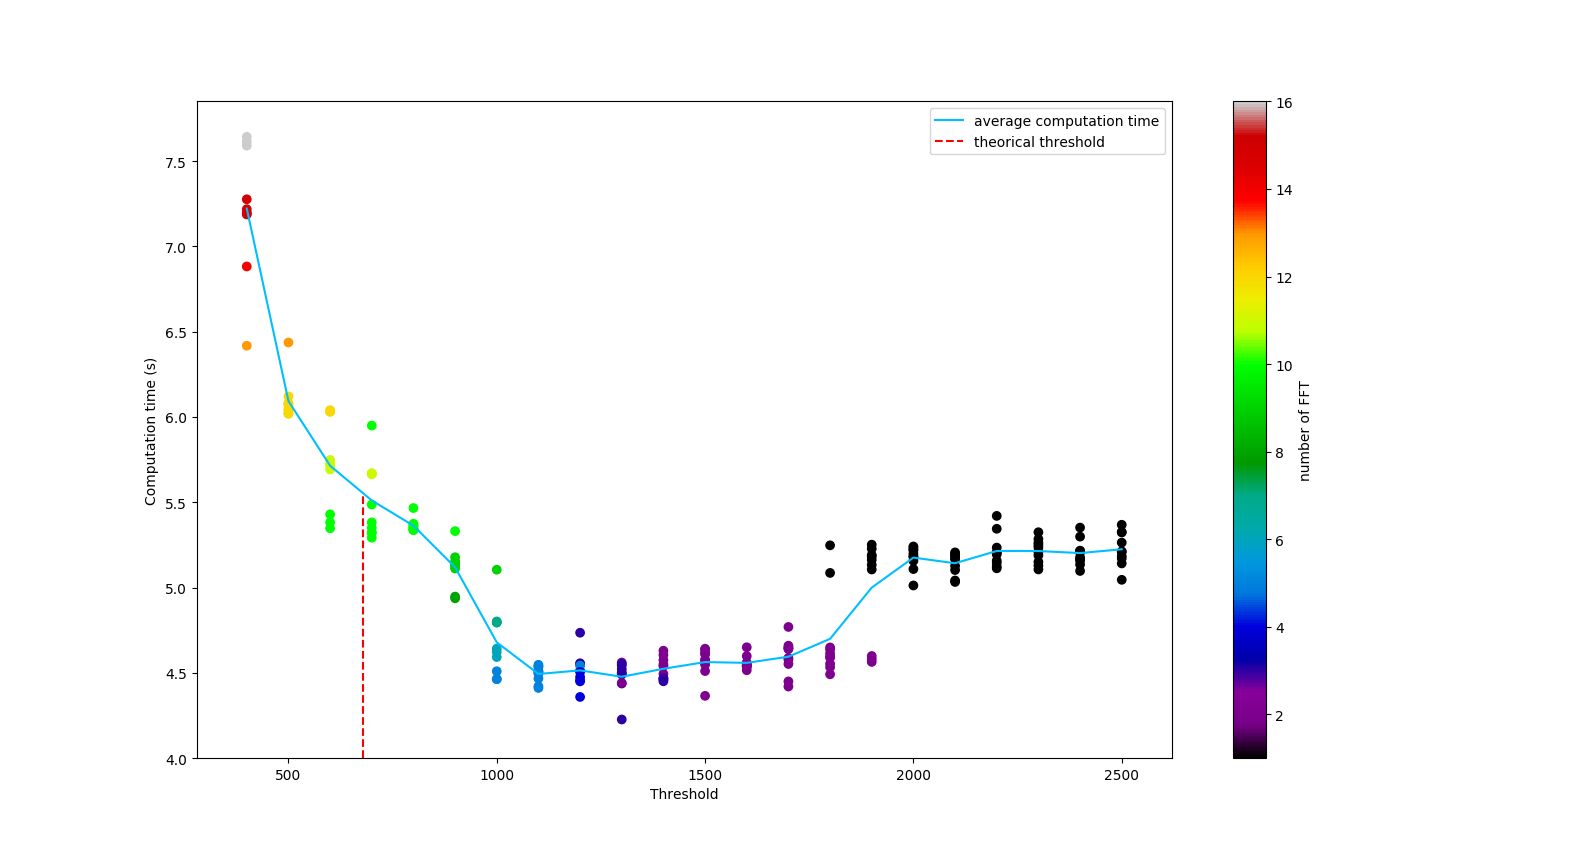
\includegraphics[scale=0.45]{./figures/ExHDThreshold.png}
\caption{Algorithm execution time for a $8$ millions letters English text
and English pattern of $0$ to $20 000$ letters.
Every point represents a run and its colour indicates the number of FFT used.
The blue curve is the average computation time of $10$ runs.
The red dotted line is the $\sqrt{m \log n}$ paper's threshold.}
\label{ExHDThresh}
\end{figure}


For a pattern of $20 000$ letters, the minimal computing time is on average $4,48$ seconds,
with a $1300$ letters threshold,
while the theoretical $\sqrt{m \log n}$ threshold was $678$ letters.
This new threshold pushes the algorithm to use $2$ or $3$ FFT.

All our tests with real patterns of different sizes produce this kind of curve:
a fast descent (up to $1100$ in the figure \ref{ExHDThresh})
then a flat section (from $1100$ to $1700$) and a small increase (from $1700$).
The flat section is represented by all the thresholds inducing an average computing time
which doesn't exceed the minimum computing time plus $0.03$ seconds.
The optimal threshold is in the flat section.
As a lucky random pattern can improve the average computation time
(as the fastest one with the $1300$ letters threshold),
we choose not to fix the threshold now, but give a range of the best threshold:
the flat section of the curve.

We ran the previous program on the $8$ millions letters of English text and patterns of increasing size
to estimate the optimal threshold depending on the pattern size.
We computed the average computation time of $50$ runs for each pattern and threshold sizes.

The figure \ref{ExHDThreshAll} shows the results on patterns of inscreasing size.
The light blue curve was made by taking the flat section's left end, 
the dark blue curve is the flat section's right end.
% Each curve represents a flat section's end of the threshold curve:
% the left end is the minimum curve, the right end is the maximum curve. 
For example in the $20 000$ letters pattern (figure \ref{ExHDThresh}),
the left end is the $1100$ letters threshold,
the right one is the $1700$ letters threshold.
We indicated the number of FFT used when the threshold is between the two thresholds.



\begin{figure}[h]
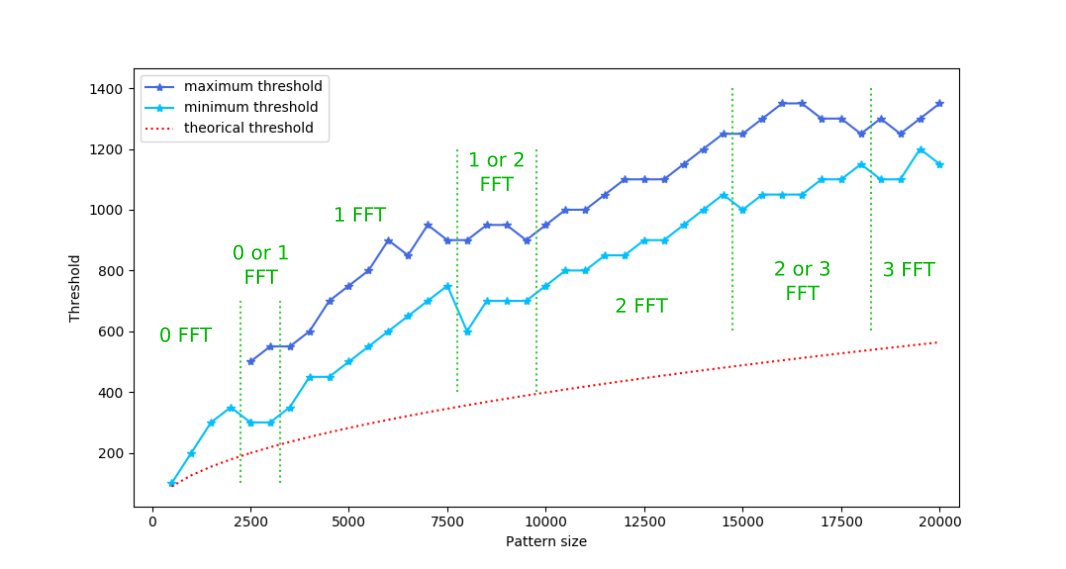
\includegraphics[scale=0.56]{./figures/ExHDThresholdAll.png}
\caption{Exact Hamming distance algorithm
running on a $8$ millions English text.
For a given pattern size,
a good threshold to use is between the two blue curves.
The number of FFT used is indicated in green.
The dotted red line indicates the $\sqrt{m \log n}$ paper's threshold.}
\label{ExHDThreshAll}
\end{figure}


The threshold should be higher for every size of pattern.

We found this kind of figure for every size of English text.

For an English text of $8$ million letters and a $20 000$ English letters,
the algorithm runs now in $4.5$ seconds, 
when it ran in $5.7$ seconds with the $\sqrt{m \log n}$ paper's threshold.

\subsubsection*{Algorithm utilisation: comparion with the naive algorithm}

\textcolor{red}{Enought??}

We recommend to use the exact Hamming distance algorithm rather than the naive algorithm
when $\sigma$ is small or when we have long patterns. \textcolor{red}{how much ??}


\subsection{approximate Hamming distance}

\subsubsection*{Implementation}



We used the following random function to map the letters:
Select randomly a primary number $p$ greater than the alphabet size $\sigma$.
Then select randomly two numbers $a$ and $b$ smaller than $p$.
Every integer $i$ representing a letter is mapped to the number
$a * i + b \equiv \pmod p \equiv \pmod \sigma$.
We used the \textit{random()} function of \textit{stdlib.h}
and generate a new seed for every mapping.
We saved the $1200$ first prime numbers in a file, loaded at the beginning of the program.


We use our optimised version of the exact Hamming distance algorithm
running in $O(n \sqrt{m \log n})$ times
rather than the algorithm $O(\sigma n \log n)$ one mentionned in the paper.
The figure \ref{AppHDComp} shows how much time we save by using this algorithm
when $\epsilon$ changes.


% We implemented two Hamming distances in the approximate algorithm.
% The first one doing $\sigma$ FFT and running in $O(\sigma n \log n)$ times,
% the second one presented here, using an optimal number of FFT,
% depending of the letters frequency and running in $O(n \sqrt{m \log n})$ times.
% We already know that the second algorithm is faster
% and the figure \ref{AppHDComp} shows the computation time of the approximate algorithm
% when we use each Hamming distance algorithms.


\begin{figure}[h]
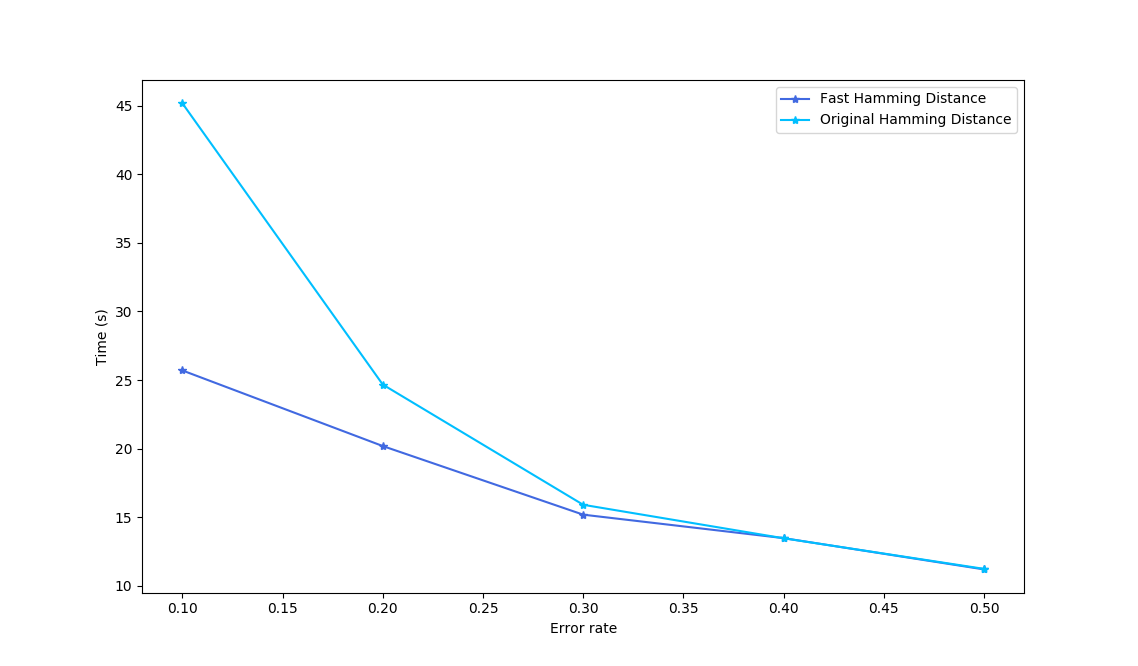
\includegraphics[scale=0.45]{./figures/appHDCompareNaive.png}
\caption{Comparison of the execution time between the optimised $O(\sigma n \log n)$ exact algorithm
(Fast Hamming distance)
and the $O(n \sqrt{m \log n})$ algorithm (Original Hamming distance).
The algorithms ran on a $8$ millions letters English text and a $5000$ letters pattern.
}
\label{AppHDComp}
\end{figure}

In the figure, when we have $\epsilon > 0.3$,
the optimum number of FFT is equal to the number of letter in the mapped text,
inducing equal running times.

We will use the $O(n \sqrt{m \log n})$ optimised version of the exact Hamming distance
algorithm in the later tests.
% rather than the $O(|\Sigma| n \log n)$ one presented in the paper.


\subsubsection*{Execution time}

This algorithm was tested on texts of $8$ millions letters,
a $10 000$ letters pattern and $\epsilon = 0.2$.

On a DNA text, the algorithms runs in around $30$ seconds.
On a English text, it runs in around $45$ seconds.
Those computations times are $10$ time slower than the exact Hamming distance algorithm,
due to the $22$ loop iterations.

We compared the approximate's results to the exact's results
and found that this algorithm approximates the Hamming distance by $\epsilon = 0.13$.


\subsubsection*{What does $2/\epsilon$ means?}

The table \ref{TableEpsilon} shows the number of letters in a text
when we use a $h: \Sigma \rightarrow \{1, 2, \ldots, 2/\epsilon\}$ mapping function.
It helps us calculate the number of FFT used in the approximate algorithm.


\begin{table}[h]
\centering
\begin{tabular}{|c|c||c|c||c|c|}
\hline
$\epsilon$ & $2/ \epsilon$ & $\epsilon$ & $2/ \epsilon$ & $\epsilon$ & $2/ \epsilon$ \\ \hline
$0.7$ & $3$ & $0.2$ & $10$ & $0.06$ & $33$ \\ \hline
$0.6$ & $3$ & $0.1$ & $20$ & $0.05$ & $40$ \\ \hline
$0.5$ & $4$ & $0.09$ & $22$ & $0.04$ & $50$ \\ \hline
$0.4$ & $5$ & $0.08$ & $25$ & $0.04$ & $67$ \\ \hline
$0.4$ & $7$ & $0.07$ & $29$ & $0.03$ & $100$ \\ \hline
\end{tabular}
\caption{Values of the rounded $2 / \epsilon$.
It represents the number of different letters after the mapping.}
\label{TableEpsilon}
\end{table}


% \subsubsection*{A simple optimization}





\subsubsection*{Can we do better than $\log n$ iterations?}
\label{AppIter}

For a $8$ millions letters English text, a $10 000$ letters pattern and $\epsilon = 0.2$,
the approximate algorithm runs in  $45$ seconds,
while using $\log n = 22$ loop iterations.
The computation time can be highly reduced by decreasing the number of iterations.
Note that the output error rate must stay under the input error rate $\epsilon$.
% \textcolor{red}{a reformuler}

We checked the approximate algorithm results
while we decrease the number of loop iterations. % in a approximate algorithm computation.
The runs with $22$ loop iterations and $\epsilon = 0.2$
produces an output error rate up to $0.087$
(we took the maximum error rate of more than $100$ runs),
we can reduce the number of iterations to come closer to the input error rate.

Our tests shows that $5$ iterations are enought
for those text and pattern sizes: the output error rate stays under $0.2$,
with a maximum of $0.107$, %(for more than $500$ runs),
while the running time decreases to $16.8$ seconds.

 

\subsubsection*{How does the error rate affect the algorithm computation time?}

The algorithm ran while the pattern size and the error rate vary
and we compare its execution time to the naive algorithm.
% The pattern is a part of the text selected randomly.
The algorithm uses $5$ iterations.
The figure \ref{AppHDTempsErr} shows the computation time of the algorithm.
Each point is the average time of $20$ runs.

\begin{figure}[h]
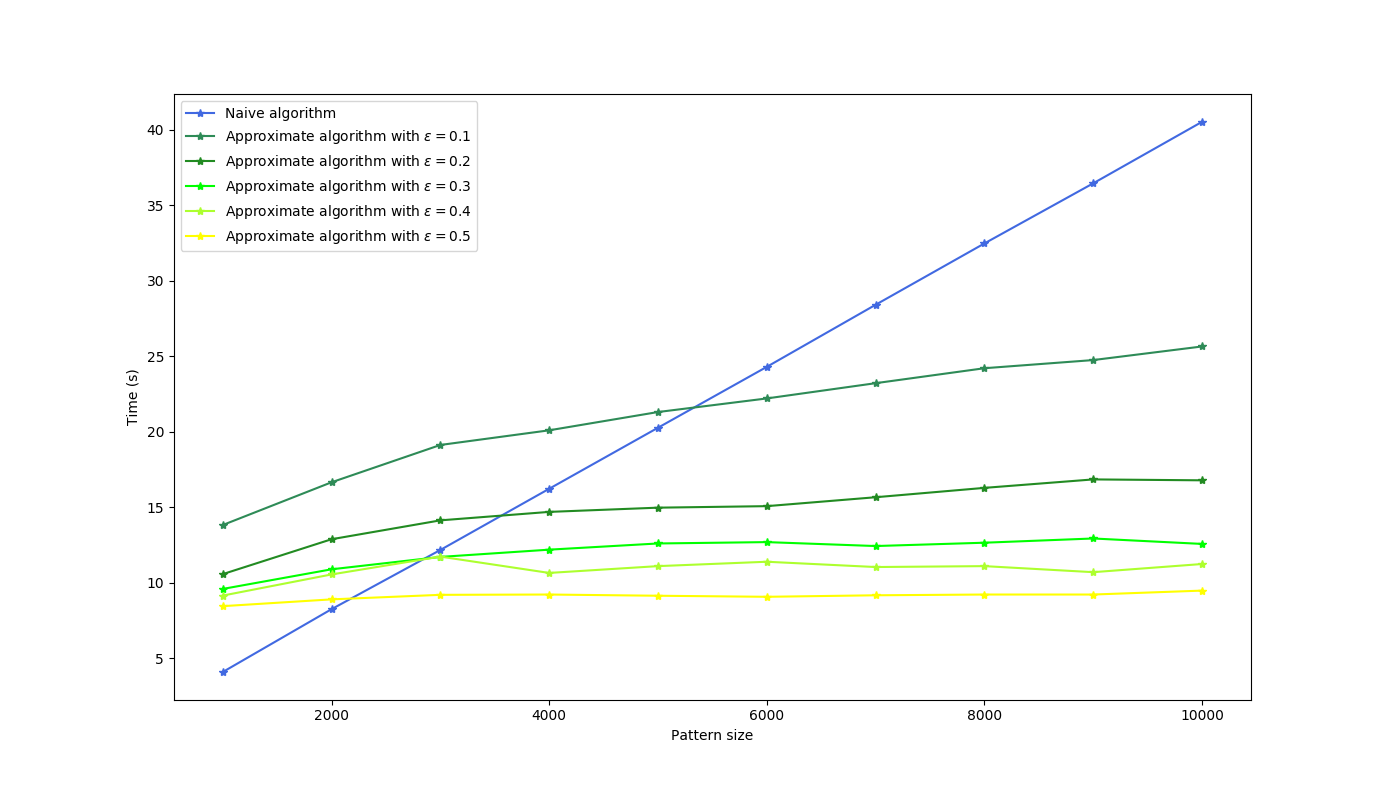
\includegraphics[scale=0.45]{./figures/appHDTempsError.png}
\caption{Approximate Hamming distance algorithm running on a $8$ millions letters of English text.
The English pattern and $\epsilon$ vary.
Comparison with the naive algorithm (blue line).}
\label{AppHDTempsErr}
\end{figure}

As expected, the smaller the value of $\epsilon$, the slower the execution time.
The naive algorithm is faster for the pattern lenght under $2000$ letters.
The curves for $\epsilon = 0.5 / 0.4 / 0.3$ are almost flat
because the mapped text is composed of $4 / 5 / 6$ letters
and the Hamming distance algorithm uses the same number of FFT.
The approximate algorithm is faster than the naive algorithm
for patterns of length up to $3500$ letters with $\epsilon = 0.2$
and patterns of length up to $5500$ letters with $\epsilon = 0.1$.



\subsubsection{Algorithm utilisation: Comparison with the exact Hamming distance algorithm}

% When should we use the approximate algorithm instead of the exact Hamming distance?

Let see the number of FFT computed in each algorithm:
the Hamming distance uses $|\Sigma|$ FFT,
while the approximate algorithm uses $c \log n 2/\epsilon$ FFT.
To use the approximate algorithm, we need to have $c \log n 2/\epsilon > |\Sigma|$. 

For our English text, we have $c 2/\epsilon * 22 > 95$.
We can use the original number of loop iterations with $c = 1$,
and be limited to $\epsilon > 0.46$,
or reduce it (without consequence on the result, see section \ref{AppIter})
with $c = 0.25$ and we can use the approximate algorithm for an error rate $\epsilon > 0.12$.

The $\epsilon$ limit changes if we have a bigger alphabet or a smaller text length.

On the other hand and looking at our tests,
it is always preferable to use the $O(n \sqrt{m \log n})$ exact Hamming distance algorithm
instead of the approximate algorithm as the exact Hamming distance uses the optimum number the FFT at all times.







\subsection{k-mismatching $1$}

\subsubsection*{Implementation}

\textcolor{red}{redo all here}

We used the data structures (SA, LCP) implementations from the \textit{geeksforgeeks} \cite{geek} web site.
The SA implementation is the fastest one to our knowledge. %not the fastest one as there are constant research to improve it.
The LCP structure is constructed in $O(n \log n)$,
slower than the $O(n)$ construction time mentionned in the paper,
but to our knowledge no $O(1)$ implementation exists.

\textcolor{red}{??}
So we will not take the SA construction time in account into this section.

\subsubsection*{Does the pattern length modify the computation time?}

On  a text of $8$ millions letters, a $1 000$ letters pattern and $5$ errors allowed,
the algorithm runs in $20$ seconds on English and DNA texts while the naive algorithm runs in $1$ second.
With patterns of $1$ million letters, the algorithm runs in $21.3$ seconds (average of $20$ runs).
The computation time doesn't increase much if we increase the length of the pattern.



\subsubsection*{Comparison with the naive algorithm and the exact Hamming distance algorithm}

The algorithm ran on a $8$ millions letters DNA text and $1 000$ letters DNA pattern
and we increase the value of $k$.
We calculated the k-mismatching algorithm's query time:
the time the algorithm uses to compute the solution when all its needed structures has been built.
The figure \ref{Kang} shows a comparison of computation times of
the k-mismatching algorithm, the naive algorithm and the optimized exact Hamming distance algorithm.
Each point represents the average time of $20$ runs.

\begin{figure}[h]
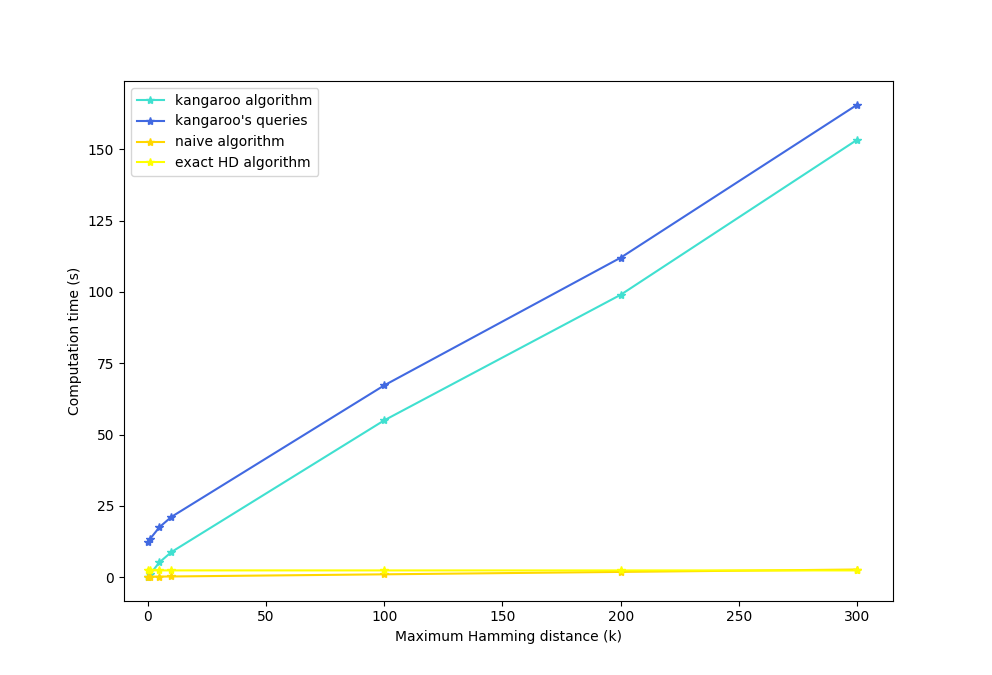
\includegraphics[scale=0.6]{./figures/Kang.png}
\caption{
Execution time of the k-mismatching algorithm $1$, exact Hamming distance algorithm and naive algorithm
when $k$ vary.
DNA text of $8$ millions letters and DNA patterns of a thousand letters.
}
\label{Kang}
\end{figure}


The full k-mismatching algorithm is always slower than the naive algorithm due to the construction time.

The computation time of the k-mismatching algorithm is better or similar to the naive one for $0$ and $1$ error.
For more than that, the naive algorithm is always faster.

The naive algorithm and the Hamming distance algorithm have similar execution time.
For DNA texts of $8$ millions letters, the naive algorithm is faster when $k < 260$,
for an English text, the naive algorithm is faster for $k < 180$. 

Most of the naive algorithm and Hamming distance algorithm computation times
are dedicated to write the result is a file ($0.83$ second).



\subsubsection*{Is there a text on which the kangaroo algorithm is faster?}

We tried to find a type of text where the kangaroo algorithm could be more efficient than the naive algorithm.
To do so, the naive algorithm should do as much comparisons as possible,
so the text and pattern should be close.
We made artificial texts where the entropy was very low:
for example, a text composed of the letters $a$ and $b$ where the $b$ are found $0.1$\% of the time.
% of the time (we call it "ratio"). In a text of 8 millions letters, a pattern of 1 000 letters, k=5 and a ratio of 0.01% (for 20 runs):

The k-mismatching algorithm runs in average in $15.7$ second, where the query time is $4.6$ seconds.
the naive algorithm runs in average in $2.7$ seconds (between $1.5$ and $4.9$ seconds)
The naive algorithm is faster even in texts with a low entropy.



\subsubsection*{Algorithm utilisation}

Note that we didn't used the fastest structure build.
So if we consider only the query time of the k-mismatching algorithm $1$,
ours tests revealed that the naive algorithm and the exact Hamming distance algorithm
are faster than the kangaroo queries is English and DNA texts for $k > 1$,
and are always faster than the k-mismatching algorithm $1$. 






\subsection{K-mismatching $2$}

% \subsubsection*{Implementation}

% We used the data structures (SA, LCP) implementations from the \textit{geeksforgeeks} \cite{geek} web site.
% The SA implementation is the fastest one to our knowledge. %not the fastest one as there are constant research to improve it.
% The LCP structure is constructed in $O(n \log n)$,
% slower than the $O(n)$ construction time mentionned in the paper,
% but to our knowledge no $O(1)$ implementation exists.


\subsubsection*{Execution time}

We executed the algorithm on $8$ million letters text and $10 000$ letters patterns.
% We used a saved patient FFT plan.

On DNA text the algorithm runs in $3.1$ seconds.
As long as $k > 4$, the $4$ letters are frequents and the running time stays constant.

On English text and $100$ errors allowed, the algorithm selects the LCP method and runs in $14.14$ second.
For $1000$ errors allowed the algorithm selects the FFT method and runs in $20.24$ seconds
(with $41$ frequent letters).
\textcolor{red}{can be better, comparison with other algorithms ??}



\subsubsection*{Algorithm utilisation}
The running time of the FFT methods depends on the number of FFT it has to compute.
The running time of the LCP method mostly depends on the structure construction time.

For a $8$ millions letters text and a $10 000$ letters pattern,
the FFT method needs around $0.5$ second per letters
while the LCP methods needs $12.5$ seconds of construction time
and up to $2$ seconds of query time.
So for those length of files, we should use the LCP methods
when the pattern is composed of more than $29$ frequent letters.

For DNA texts and other small alphabets, the FFT method should always be used.





\subsection{k-mismatching $3$}

\subsubsection*{Implementation}
We swapped the Approximate Hamming Distance algorithm used to compute the pattern period,
to the exact Hamming Distance algorithm.


\textcolor{red}{WHAAT ?}
We used the Approximate string matching algorithms instead of Karloff's algorithm.


\subsubsection*{Execution time}

We tested this algorithm on English and DNA sequences of $100 000$ letters with a $10 000$ letters pattern.
% We used our optimisations.

On the DNA text, and $k = 10$, the algorithm uses the LCP method and runs in $7.8$ seconds.
On the DNA text and $k = 300$, the algorithm uses the RLE method and runs in less than $0.1$ second.
On the English text and $k = 10$, the algorithm uses the LCP method and runs in $6.6$ seconds
On the English text and $k = 50$, the algorithm uses the RLE method and runs in $4.6$ second.

The main difference between the execution time of the runs using the RLE method %(runs $2$ and $4$)
comes from the number of different letters in the text.
In the DNA text, the $4$ letters are frequents so $4$ FFT are used,
with no additional second derivative updates.
In the English text, $6$ to $7$ letters are frequents, and we have a least $900 000$ second derivative updates.



\subsubsection*{Threshold between the RLE and FFT methods}

First, we tested the $8k$-period part to find the best threshold
used to sort the characters as frequent or infrequent.
$t$ is a threshold on the number of run a character is present in.

The execution time depends on the number of pair of run text/pattern.
We increase the number of pair of runs and compare it to a FFT execution.
See the table \ref{OptiComp}.

\begin{figure}[h]
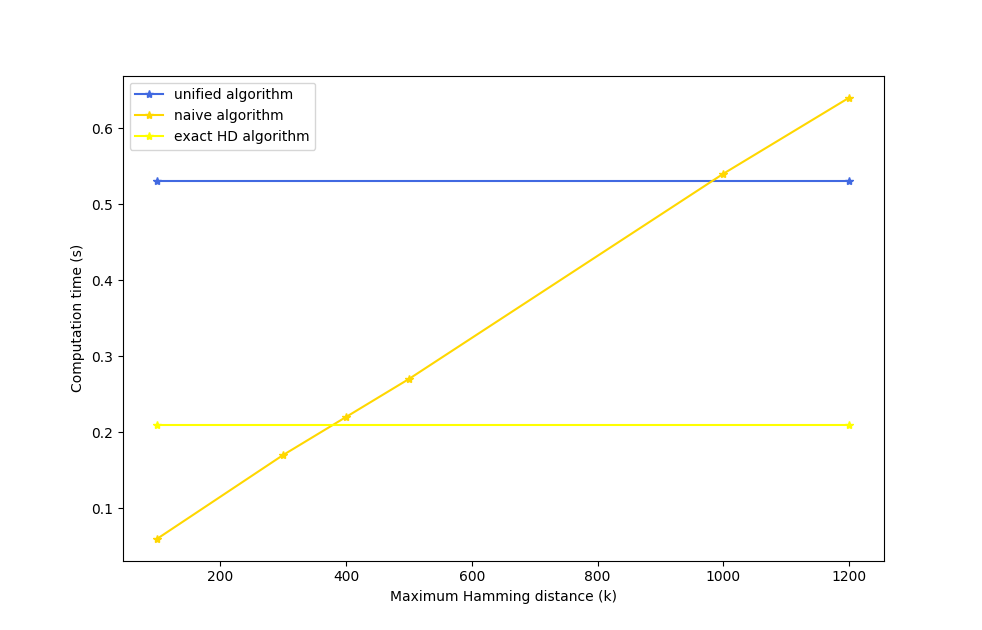
\includegraphics[scale=0.45]{./figures/OptiComparOptiNaivHD.png}
\caption{XXXX}
\label{OptiComp}
\end{figure}

The execution time of the part using the FFT includes the production of $T^*$ and $P^*$ strings
and the FFT method for one letter.
If a second letter is computed, the execution time is close to twice the time for one letter.
We used pre-computed patient plans. 

The execution time of the part using the RLE runs grows linearly with the number of pairs of runs.
This curve and the FFT for $2$ millions letters cross at $55$ millions of pair of RLE runs.   

For an execution of the k-mismatching for a $1$ million letters pattern,
the threshold between frequent and infrequent letters is $55$ millions pairs of RLE runs
(as we will use FFT on $2$ millions letters).



\subsubsection{K-mismatching $3$ vs. exact Hamming Distance: increase the number of pair of runs}

We created texts of $100$ differents letters such that we can control the number of pair of runs
between the text and pattern.

On a $1$ million letters text, a $100$ thousand letters pattern and $k = 100$,
the execution time of the exact Hamming distance and the k-mismatching are gathered in the figure \ref{Opti01FFT}.


\begin{figure}[h]
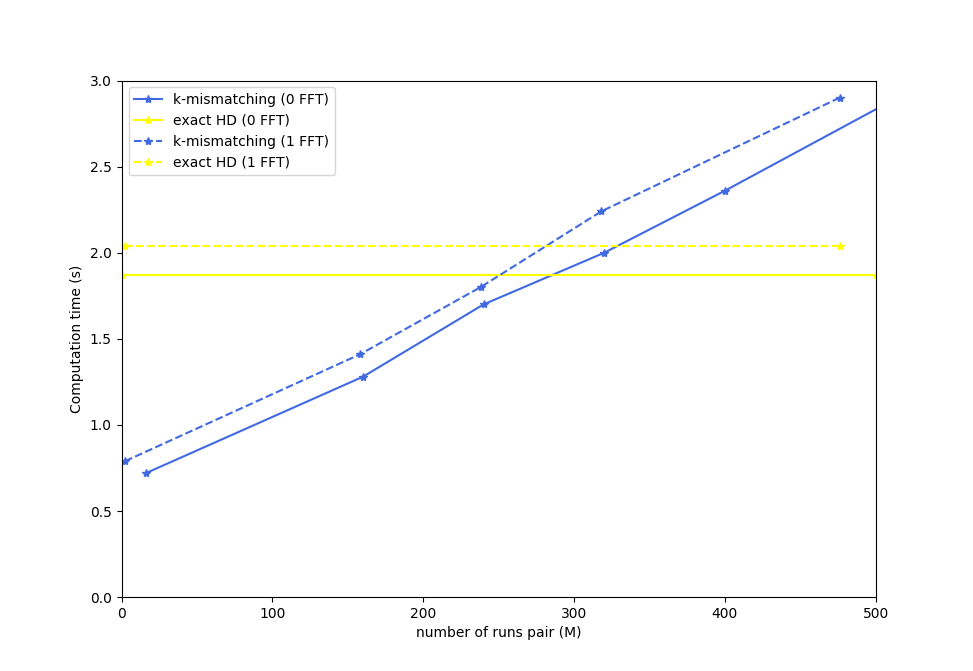
\includegraphics[scale=0.45]{./figures/Opti01FFT.png}
\caption{XXXX}
\label{Opti01FFT}
\end{figure}

In the patterns, all letters appeared with the same frequency,
but we forced the utilisation of $0$ and $1$ FFT in both algorithm.
In both cases, the execution time of the algorithms are similar around $300$ millions pairs of runs:
the k-mismatching is faster under $300$ millions pair of runs.
The same kind of curves were find for $5$ FFT and $15$ FFT, they also intersect around $k=300$ millions.



\subsubsection{K-mismatching $3$ vs. exact Hamming Distance: real files}

On a $1$ million letters text and a $100$ thousands letters pattern.

On DNA files, the exact Hamming distance algorithm runs in $0.44$ second.
The k-mismatching use the LCP method until around $k=6500$,
the LCP construction only alone needs several seconds.
When $k>6500$, the RLE method is used, the algorithm runs in $1.67$ second.
As all letters are frequent, both algorithms use $4$ FFT.
The additional computation time of the k-mismatching  comes from the period pattern calculation,
the computation of $T^*$, $P^*$ and so on.

On English text, the exact Hamming distance algorithm runs in $1.5$ second.
The k-mismatching use the LCP method until around $k=20000$,
the LCP construction alone needs several dozens of seconds.
When $k>20000$, the RLE method is used, the algorithm runs in $7.5$ second.
$18$ letters are frequent, but text and pattern aren't periodical enough to profit from the RLE method.



\subsubsection{Algorithm utilisation}
The exact Hamming Distance algorithm is always faster that the k-mismatching algorithm for short alphabet (DNA).

Text and pattern should have a good periodicity, otherwise, the LCP method is too slow.

Note that we didn't used the fastest LCP construction method.








\section*{Conclusion}
resume of results

stringipedia


ouverture et travail futur : we would like to implement Clifford's algorithm

								find/do better LCP structures implementation 





\section*{Bibliography}

\bibliographystyle{abbrv}
\bibliography{biblio}

%% Authors are advised to submit their bibtex database files. They are
%% requested to list a bibtex style file in the manuscript if they do
%% not want to use model1-num-names.bst.

%% References without bibTeX database:

% \begin{biblio}

%% \bibitem must have the following form:
%%   \bibitem{key}...
%%

% \bibitem{}

% \end{thebibliography}


\end{document}

%%
%% End of file `elsarticle-template-1-num.tex'.